%2345678901234567890123456789012345678901234567890123456789012345678901234567890
%%%%%%%%%%%%%%%%%%%%%%%%%%%%%%%%%%%%%%%%%%%%%%%%%%%%%%%%%%%%%%%%%%%%%%%%%%%%%%%%
% MAURICIO ESGUERRA NEIRA
% Ph. D. Thesis
%%%%%%%%%%%%%%%%%%%%%%%%%%%%%%%%%%%%%%%%%%%%%%%%%%%%%%%%%%%%%%%%%%%%%%%%%%%%%%%%
\chapter{Introduction}
\label{introduction} 
\bibliographystyle{nar}
%\section{RNA}
RNA plays  a primordial role  in life, and  perhaps also in  the early
history   of  its   origins  \cite{woese1967,   crick1968,  orgel1968,
  orgel2004}.  In molecular  biology RNA  is a  central player  in the
transcription and  translation steps of  what is known as  its central
dogma, i.e., DNA  makes RNA (via transcription) and  RNA makes protein
(during  translation).   %A first  RNA  step  transcribes the  genetic
message %written  in the DNA  alphabet, to the RNA  alphabet producing
mRNA.   In the last  decade of  the twentieth  century Fire  and Mello
\cite{fire1998} found that RNA also plays a role previously thought to
be the  job of proteins. That  is, RNA can  regulate translation using
non-coding RNA's  (ncRNA's).  Another fundamental  discovery about RNA
came in  2000 with  the elucidation of  the structure at  atomic level
detail of  a large non-coding RNA,  the ribosome \cite{schluenzen2000,
  ban2000, wimberly2000}.

Since its very beginnings,  structural understanding of RNA has proven
to be a very complex problem. It was not until 1956, three years after
the  famous  \textit{Nature} triad  of  papers  by  Watson and  Crick,
Wilkins,    Stoke,   and    Wilson,   and    Franklin    and   Gosling
\cite{watson1953a,  wilkins1953, franklin1953} on  the double-stranded
structure of DNA, that Alex Rich and David Davies were able to produce
double-stranded   RNA  from   polyriboadenylic   acid  (poly-rA)   and
polyribouridylic acid  (poly-rU) to produce a  neatly difracting X-ray
pattern typical of  a double-helical structure. It was  not until 1965
that Robert Holley  was able to obtain the  complete sequence of yeast
alanine tRNA,  and also its  secondary structure from cleavage  of the
whole structure  into smaller fragments \cite{holley1965},  and it was
only in 1973,  that the first complex, but  small, tRNA structure, was
solved at full  atomic detail \cite{robertus1974, kim1974, stout1976}.
Fifty  seven   years  have  passed   since  the  description   of  the
double-helical structure  of DNA, but still RNA  faces more challenges
with  the possibility of  finding a  whole new  zoo of  non-coding RNA
structures \cite{weinberg2009}, and  the possibility of new engineered
ones \cite{severcan2009}.

\section{RNA chemistry}
\label{sec:rnachem}
RNA is  a polynucleotide  chain, that is,  a polymer  whose monomeric
unit  is the  nucleotide.  The  nucleotide unit  is composed  of three
chemically distinct  entities: base,  sugar, and phosphate.  The bases
can be  of two types, purines  (R), i.e. adenine (A)  and guanine (G),
and  pyrimidines (Y), i.e.  cytosine (C)  and uracil  (U) as  shown in
Figure~\ref{fig:chemistry1}.
\begin{figure}
\centering
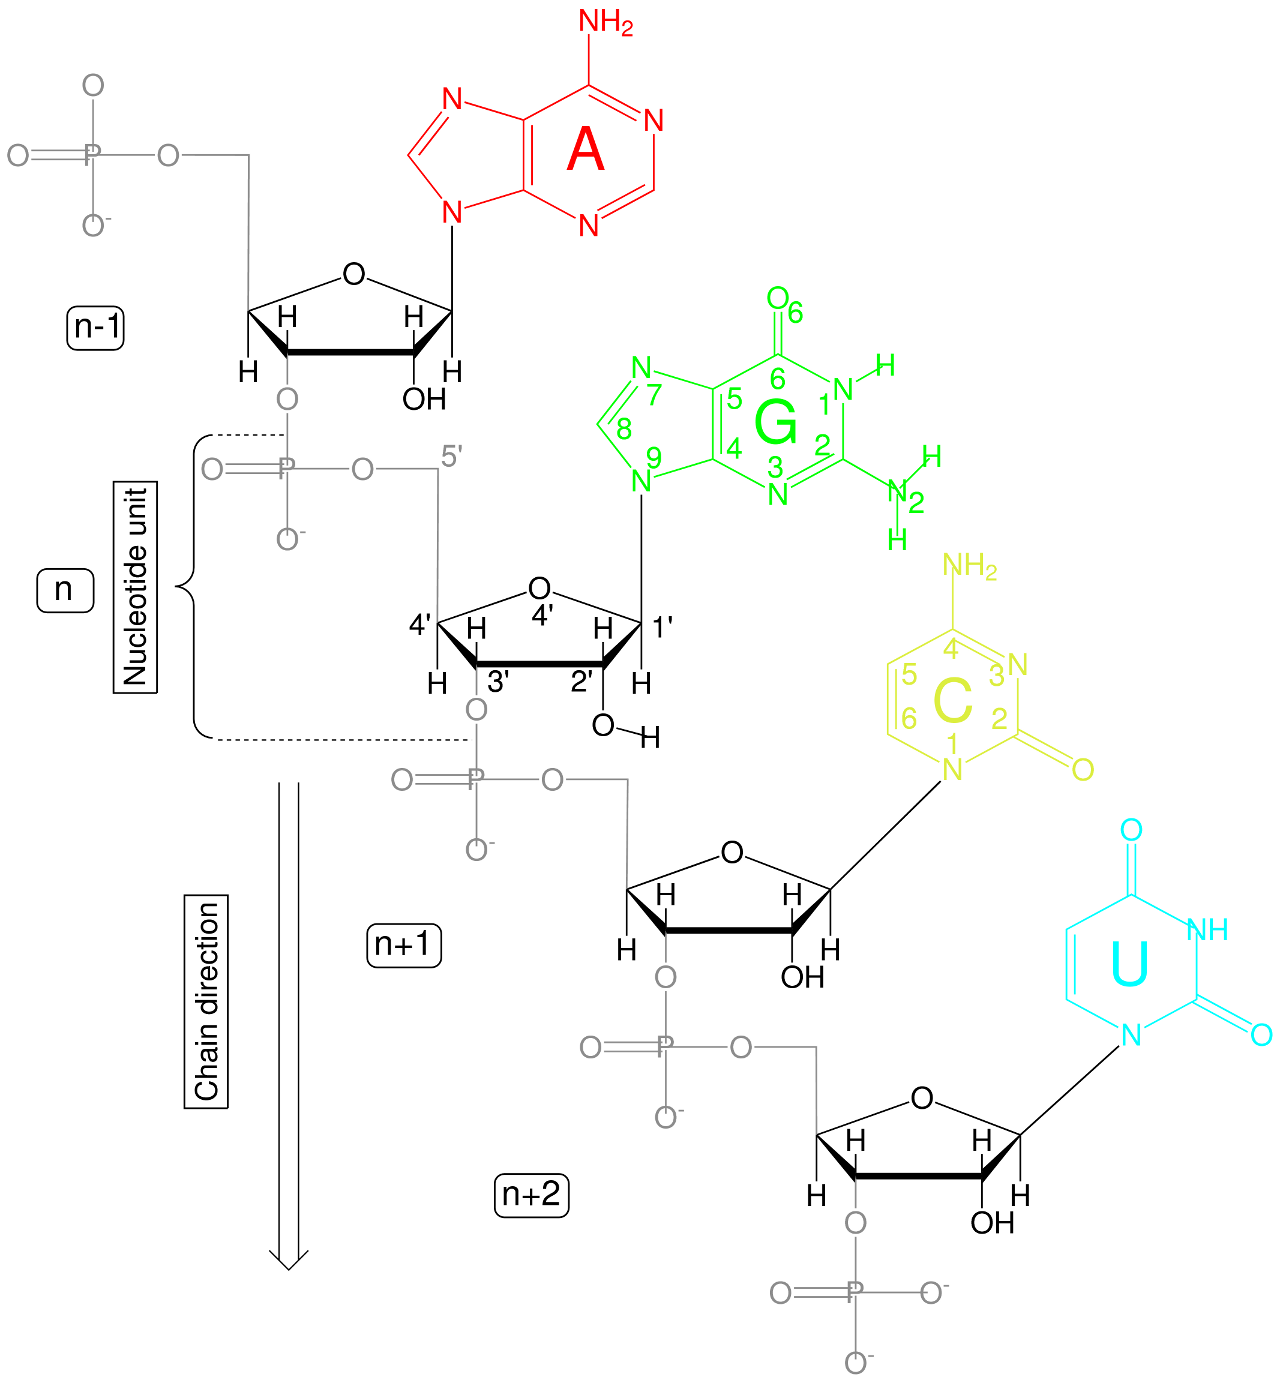
\includegraphics[scale=0.8]{Chapter1/chemistry1b.png}
\caption{A  single strand  of  RNA drawn  in  the 5$'$  to 3$'$  sense
  showing the  three chemical entities which compose  it- base, sugar,
  and phosphate.  The four bases (A, G, C, U) are colored according to
  the  NDB  (Nucleic  Acid  Database)  convention  \cite{ndburl},  the
  phosphate is colored gray, and the sugars black. The bases G, and C,
  and the furanose  sugar attached to the G  are numbered according to
  the IUPAC  rules \cite{iupac1983}. This  figure is an  adaptation of
  Figure 2.1,  in Wolfram Saenger's book, "Principles  of Nucleic Acid
  Structure" \cite{saenger1984}.}
\label{fig:chemistry1}
\end{figure}  

The  heterocyclic bases  can form  a diversity  of base  pairs through
hydrogen bonding and associate in  at least 28 distinct classes, first
proposed   by   Saenger    \cite{saenger1984}   and   illustrated   in
Figure~\ref{fig:saenger28}. A system of base-pair nomenclature, which
conforms  to  Saenger's  groups,  has  been  developed  by  Lee-Gutell
\cite{lee2004}, Leontis-Westhof \cite{leontis2002b}, and Lemieux-Major
\cite{lemieux2002} in order to classify the arrangements of bases seen
in high-resolution structures.

\begin{figure}
\centering
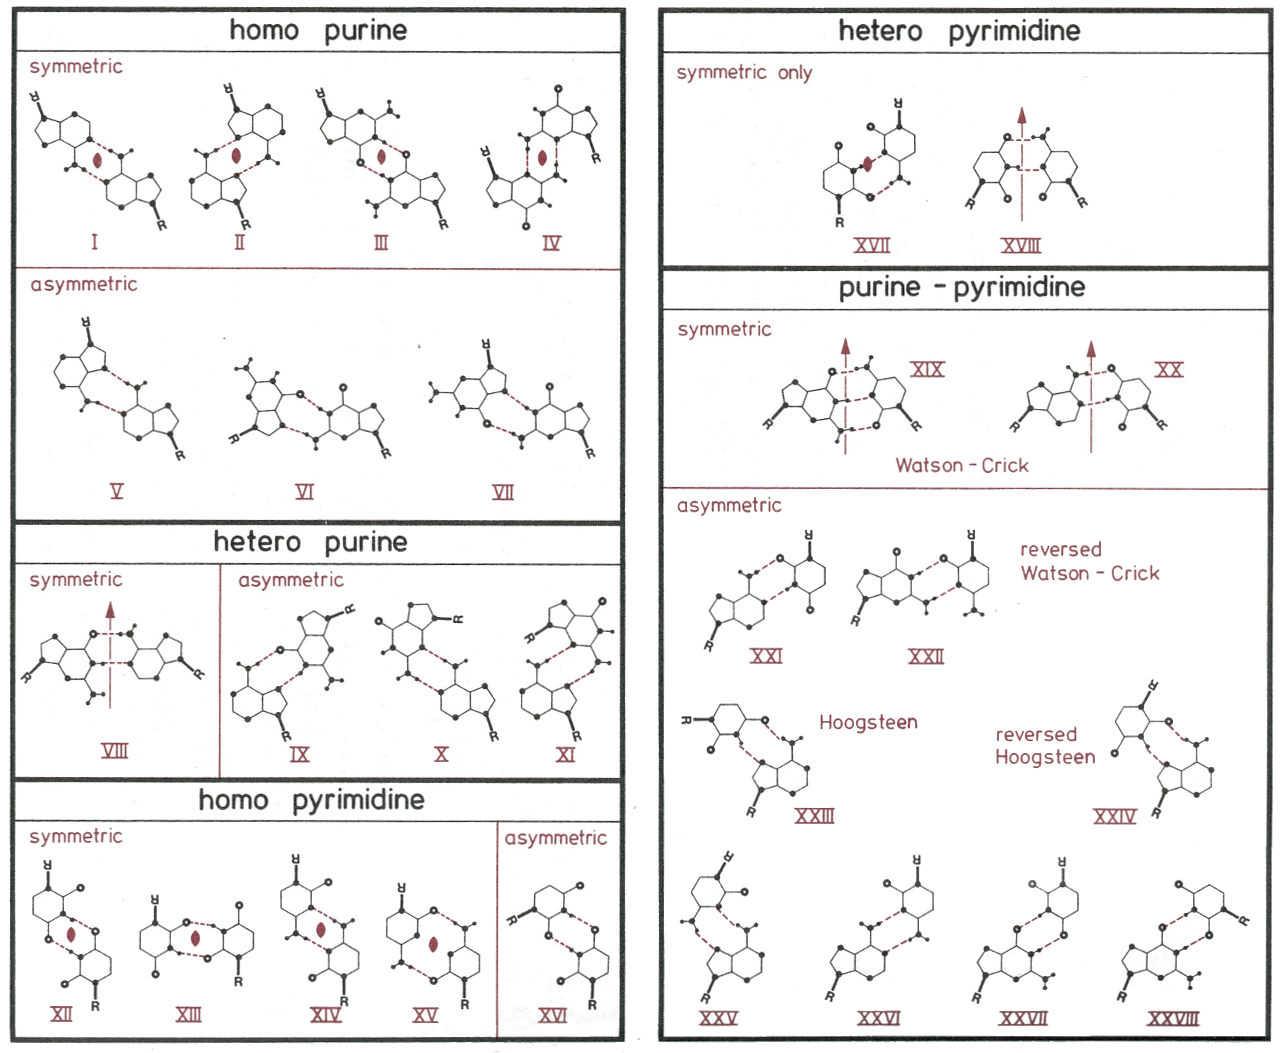
\includegraphics[scale=3.8, angle=90]{Chapter1/saenger28c.png}
\caption{Saenger base-pairing classes, reproduced with permission from
  his       book,        "Principles       of       Nucleic       Acid
  Structure". \cite{saenger1984}.}
\label{fig:saenger28}
\end{figure}  

The other non-covalent interactions which are common to the nucleotide
bases  are those  of  stacking through  London  dispersion forces  and
electrostatic  interactions.   It  has  been hypothesized  that  $\pi$
electron  interactions  could  also  account for  stacking,  but  very
precise quantum  calculations \cite{sponer1996, sponer1997}  have show
otherwise thus far.

The sugar and  phosphate groups can adopt a  variety of conformations,
typically defined by the values of the torsion angles described by the
planes formed by four succesive atoms.   In the case of the sugar, the
torsion  angles are constrained  by the  closure of  the five-membered
ring  to  distinct  ranges  corresponding to  two  principal  puckered
arrangements in  which one  or two of  the five  atoms lie out  of the
plane defined  by the other four  or three atoms.   The prefered sugar
pucker in RNA is the C${3'-\textrm{endo}}$ form, but in cases where a
base  intercalates  between two  sequential  bases,  the sugar  pucker
frequently   change   to   the  less-prefered   C${2'-\textrm{endo}}$
conformation.  Standards to  describe the conformations resulting from
the specific sets  of torsion angle values which  sugars and phosphate
can  attain  have  been  developed   and  can  be  seen  in  textbooks
\cite{saenger1984},  on  the  web  \cite{jenaurl}, and  in  the  IUPAC
recommendations  \cite{iupac1983}.   We  refer  the  reader  to  these
sources for  a more detailed  description, and limit ourselves  to the
brief    description    of    these    torsion   angles    shown    in
Figure~\ref{fig:puckersbbone}.

\begin{figure}
\centering
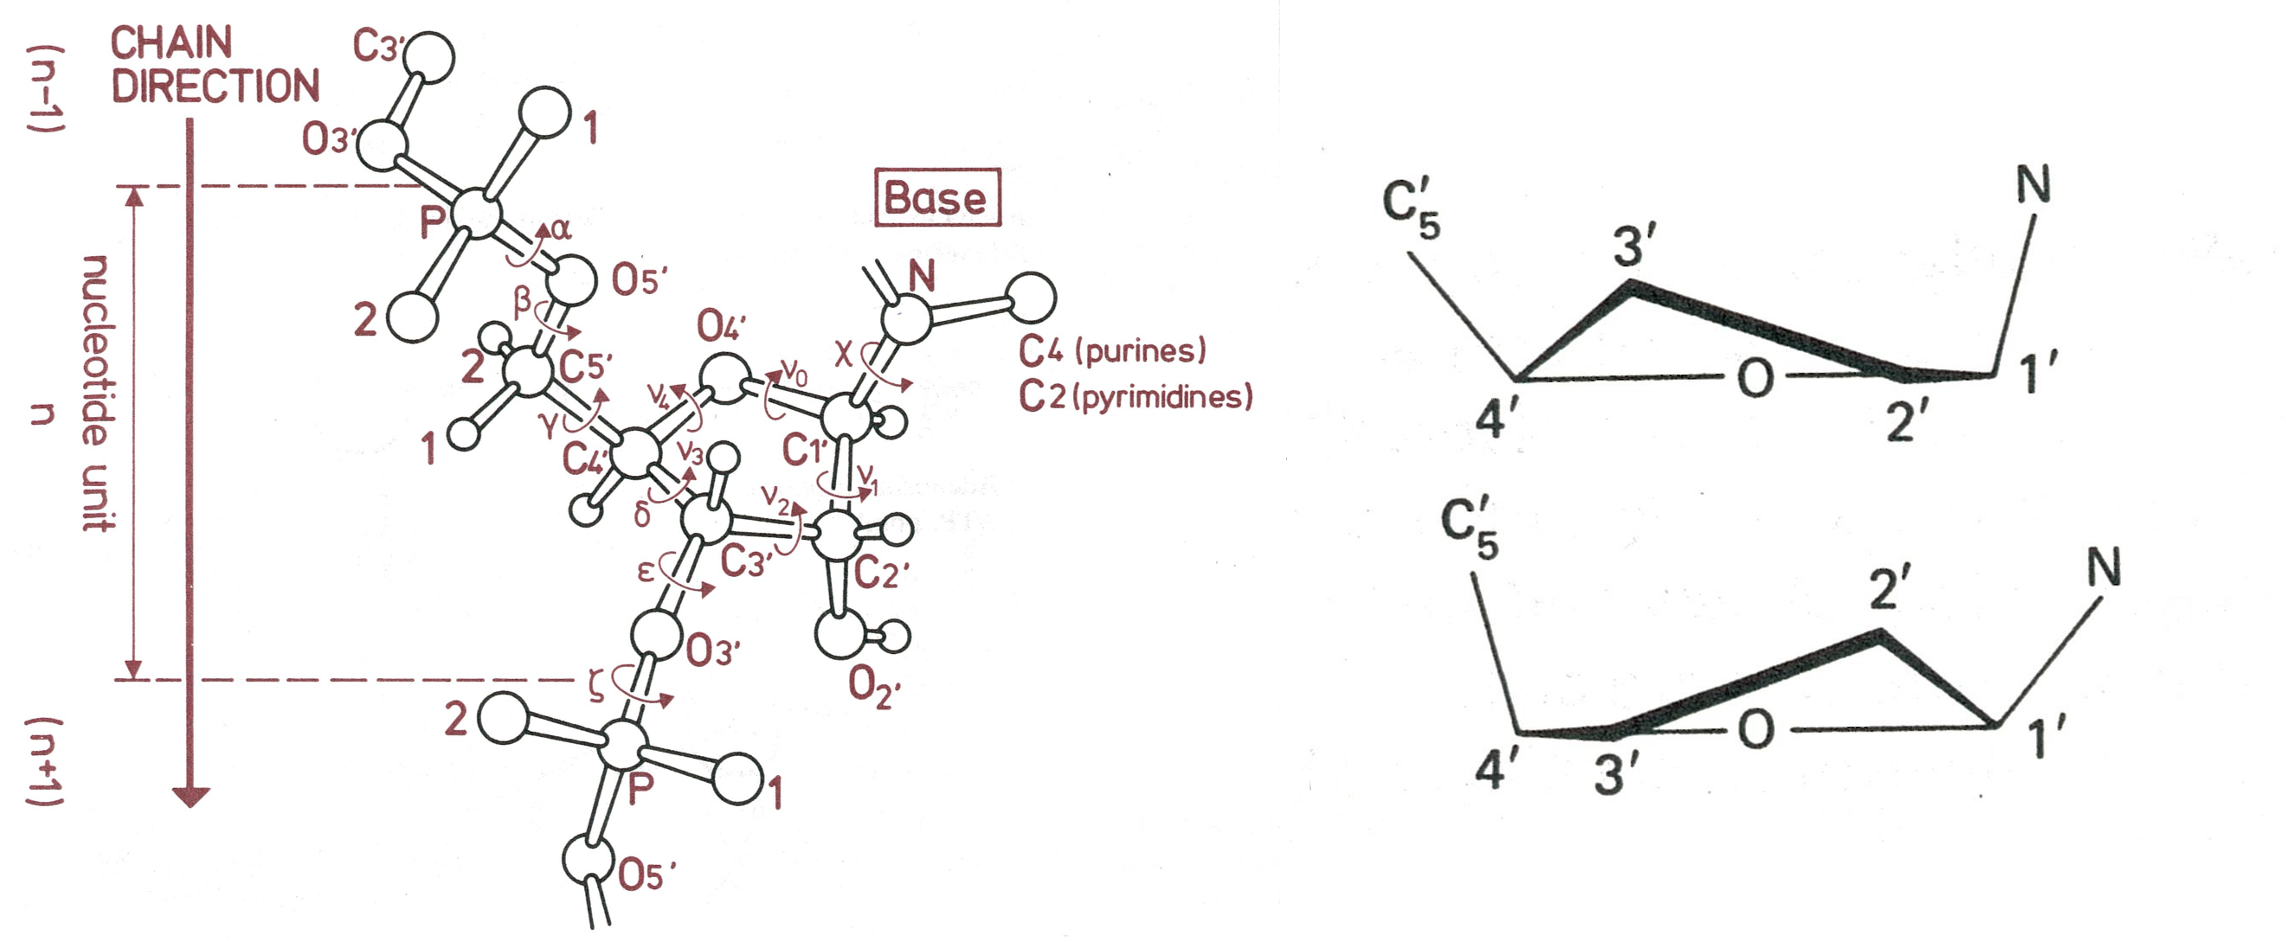
\includegraphics[scale=1.8, angle=0]{Chapter1/torsions.png}
\caption{\textbf{Left:}  Sugar, and  sugar-phosphate  backbone torsion
  angles. \textbf{Right:}  The most common  sugar pucker conformations
  in RNA, that  is, C${3'-\textrm{endo}}$ and C${2'-\textrm{endo}}$,
  reproduced  with permission from  Wolfram Saenger's,  "Principles of
  Nucleic Acid Structure". \cite{saenger1984}.}
\label{fig:puckersbbone}
\end{figure}  

%A-RNA 
%Loops
%Reference:
%Pure \& Appl. Chem., Vol.55, No.8, pp.1273—1280, 1983
%\url{http://www.fli-leibniz.de/ImgLibDoc/nana/IMAGE_NANA.html}


\section{RNA folding}
The first  high-resolution X-ray\index{X-ray} structure  of RNA larger
than  a dinucleotide  was  that of  yeast  phenylalanine transfer  RNA
(tRNA$^{\textrm{Phe}}$), solved at 3{\AA}in 1974 \cite{robertus1974,
  kim1974, stout1976}.  Thirty six years later there are two orders of
magnitude more structural information about RNA \cite{noller2005}, and
new information from non-coding RNA's is expected \cite{weinberg2009}.
This   fact   and  the   discovery   of  ribozymes   \cite{kruger1982,
  takada1983}, which are catalytic RNA molecules, has renewed interest
in  solving  the  RNA  folding\index{RNA folding}  problem,  that  is,
starting    from    the    primary    sequence,    finding    in    an
automated\footnote{The  term   automated  is  used  here   to  mean  a
  theoretical model of tertiary  folding, which could use experimental
  measures of secondary structure association in the same way that the
  traditional  secondary   structure  folding  model  \cite{zuker1989,
    hofacker1994}  uses  the  Tinoco-Uhlenbeck dinucleotide  postulate
  \cite{borer1974} to find total free energies That is, it is assumed
  that the total free energy of the RNA polymer is the sum of the free
  energies of the individual base-pair steps which constitute it.} way
the  native three-dimensional  structure of  an RNA  molecule  and the
folding pathway  that it follows.  The  RNA folding\index{RNA folding}
problem is usually  seen as analogous to the  protein folding problem,
due  to both  the  discovery  of  the  enzymatic   behavior  of  RNA
\cite{kruger1982, takada1983} and the complicated folding of large RNA
molecules  \cite{batey1999}.  To  take  advantage of  this analogy,  a
unified conceptual  framework for describing RNA  and protein folding,
called the kinetic partitioning mechanism (KPM), has been developed by
Thirumalai  and Hyeon  \cite{thirumalai2005}. This  and  other methods
used to characterize RNA and protein folding depend upon the partition
function  used  to describe  the  correct  conformational ensemble  of
folded,  partially  folded,  and unfolded  structures  \cite{chen1995,
  chen1998, thirumalai1996} of either protein or RNA.

\section{Is RNA folding a hard or easy problem?}
There  are  two trains  of  thought  regarding  the mechanism  of  RNA
folding.  One  states that  RNA folding is  less complex  than protein
folding  \cite{tinoco1999} because  RNA is  made up  of a  four-letter
alphabet of similar  nucleotide units instead of a  20-letter alphabet
of  dissimilar   amino  acids.   Therefore  the   number  of  possible
sequential  combinations  is smaller.   It  is  also  well known  that
secondary and  tertiary interactions can  be separated in the  case of
RNA  by the absence  or presence  of Mg$^{2+}$  \cite{rangan2003} (see
Figure~\ref{fig:folding}), and  that the secondary structure motifs
of RNA are more limited  in  number  than  those  of protein. By contrast
secondary  and tertiary elements are not as easily separable in
proteins.
\begin{figure}[ht]
\centering
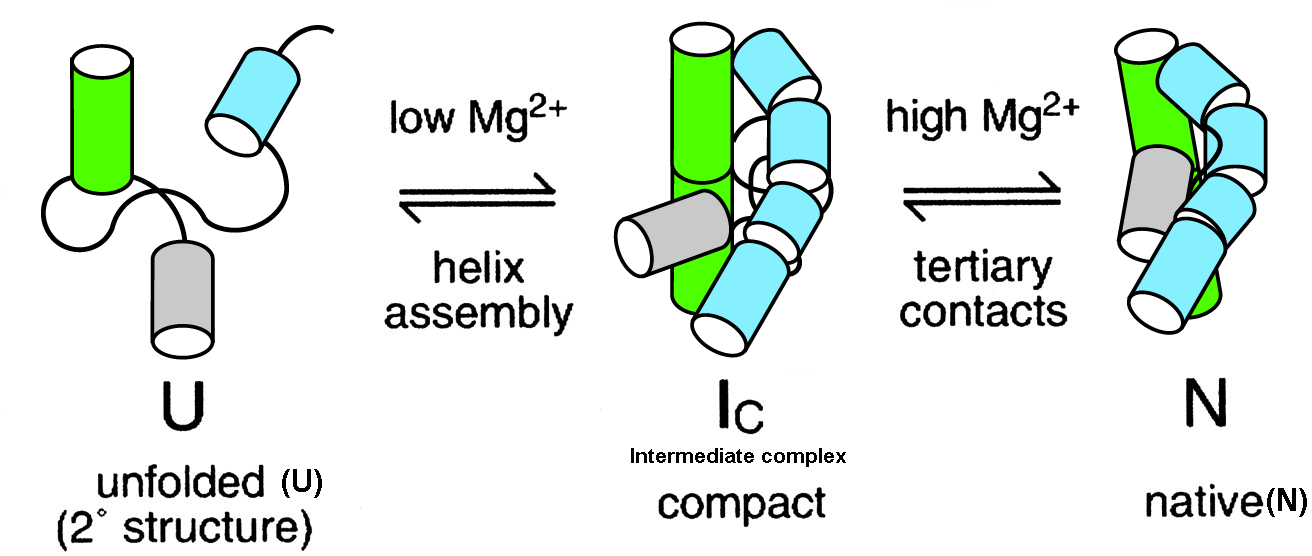
\includegraphics[scale=0.3]{Chapter1/rangan2003pnas.png}
\caption{Separation  of  secondary and  tertiary  interactions in  RNA
  \cite{rangan2003}. Double helical secondary structure represented by
  individual  cylinders and  tertiary interactions  by  association of
  cylinders. Color coding stands  for separate helical regions of RNA,
  and  the connecting  black  strings represent  single stranded  loop
  structures.   The   cartoon  corresponds  to   the  Mg$^{\text{2+}}$
  dependent folding  of the  \textit{Azoarcus} ribozyme, where  at low
  magnesium  ion  concentrations an  intermediate  and somewhat  loose
  ensemble  of conformations  denoted by  I$_{\text{C}}$ is  formed by
  association  of   helical  segments.   At   higher  Mg$^{\text{2+}}$
  concentrations the  helices arrange into a more  ordered and compact
  structure which is catalitically active and is denoted as the native
  state N.}
%% Note that Dr. Olson asks what the colors in cylinders mean.
%% Answer: They mean nothing. Perhaps only that the cyan stands for
%% the helical structures making a pseudo-knot, that is, P7 and P3.
\label{fig:folding}
\end{figure}

The  other point of  view says  that RNA  folding can  be at  least as
complex as protein folding \cite{moore1999a, sorin2004} since there is
no such thing  as hydrophobic burial of regions of RNA  as in the case
of  proteins.   Instead, the  electrostatic  problem  stemming from  a
complex charged backbone and polar base side groups must be dealt with
in the case of RNA.
% The case of the electrostatic treatment of the backbone is lacking
% here, most likely WKO wants me not to ignore our own Gerald Manning
% tinoco 1999 says this must be an easy to solve problem since we can
% do the electrostatics for it easily
For instance,  the interactions of  the RNA polyanionic  backbone with
water  and cations  \cite{klein2004a}  are not  easily simulated  with
explicit   solvent  models   like those used to treat   proteins.  The
aforementioned interactions of RNA  need to be modeled implicitly, and
must aim to describe long dynamic processes of the order of seconds to
minutes,  in  contrast   to  the  typical  time  scales   of  tens  of
microseconds associated with protein folding.
% Remember that this means that a explicit calculation for RNA would
% be prohibitively large.

Although   secondary   and  tertiary   structure   can  be   separated
experimentally, there have been few theoretical efforts to account for
the  folding  of  RNA  from  a random  sequence  of  nucleotides  into
secondary structures and tertiary  structures. What little is know has
been  investigated at  low resolution.  Stephen Harvey  and associates
have   simulated   the   folding   of   yeast   tRNA$^{\textrm{Phe}}$
\cite{malhotra1990}  and  the  assembly  of  the 30S  subunit  of  the
ribosome \cite{stagg2003} at various levels of detail, initially using
only one pseudoatom  per helical region, and later  one pseudoatom per
nucleotide.  Recently  Fran\c{c}ois  Major's  group  at  Montreal  has
proposed a pipeline of two  computer algorithms to study RNA structure
\cite{parisien2008}.   One    pipeline   makes   secondary   structure
predictions, and the  other assembles 3D structures based  on the best
scoring secondary structures.
% Note for presentation ==> Include figure 1 in Malhotra-harvey paper
% Look at what says in folding.stanford.edu/science.html Also take
% into account Biophys J. V.88 2516-2524 for the case of having to
% think of water in the folding problem.
By contrast,  in the case of  proteins many groups  have simulated the
transition  from  secondary  to  tertiary  structure,  including  some
calculations which  account for the  strong coupling of  secondary and
tertiary  structure   \cite{westhead1999,  gerstein2003,  meiler2003}.
This type of work is  often referred to as protein structural topology
and there is no counterpart for RNA.

%The seminal paper here seems to be the one of liphardt in 2001 for
%rna unfolding
\section{Experimental folding techniques}
Traditionally   RNA   folding  and   unfolding   have  been   followed
calorimetrically  and spectroscopically as  a function  of temperature
and cation concentration  \cite{bloomfield2000, boots2008}. While this
approach  works well  for studying  two-state  folders, \textit{i.e.},
structures  which populate  only two  states (native  and  melted), in
general RNA's  are not  two-state folders. RNA  seems to go  through a
rugged  free  energy landscape  of  conformations  in  the process  of
folding \cite{zhuang2003}.  The  experimental solution to this problem
is offered  by single-molecule techniques  like fluorescence resonance
energy transfer (FRET) and  mechanical micromanipulation, in which the
ends of RNA  are attached to micron sized beads  that are then pulled
apart  and  monitored  with  a laser  light  trap  \cite{liphardt2001,
  onoa2004,  tinoco2004, hyeon2005}.  In  the case  of single-molecule,
force-induced   unfolding,  state   transitions   often  occur   under
non-equilibrium  conditions, thereby  making it  difficult  to extract
equilibrium  information from the  data. Bustamante, Tinoco,
and associates have shown that by using the Crooks fluctuation theorem
\cite{crooks1999},  one  can deal  with  such  cases  and extract  RNA
folding    free     energies    from    single-molecule    experiments
\cite{collin2005}. %Recently an alternative solution to this problem has
%been proposed by Thirumalai and associates based on single-molecule
%force-quenching experiments, by using a so called  de Genes "expanding
%sausage model" \cite{hyeon2009}.

%\subsection{RNA Folding in Vitro vs in Vivo vs in Silico}
% It still is to be seen whether the following is relevant or not
% This single molecule information is
% collected in-vitro and not in-vivo, which is actually the ultimate
% problem aimed for prediction, there's quite a lot of evidence for
% different folding states reached in one case and not the other and
% viceversa \cite{sosnick2003, schroeder2002} but still a first step
% towards understanding in-vivo folding is in-vitro and in-silico
% experimentation.


\section{RNA simulations}
Network  and molecular  mechanics-molecular  dynamics (MM-MD)  methods
provide  useful  information  relevant  to the  RNA  folding-unfolding
problem, especially  for describing fluctuations away  from the native
conformation.   Gaussian network  models  \cite{y_wang2004, bahar1998,
  wang2005}, which  treat RNA  at less than  atomic detail,  have been
used to describe  the global motions of large  RNA structures like the
ribosome.  Examples  of the  predicted normal modes  of motion  of the
ribosome  can  be  seen  at   the  Robert  Jernigan  group  web  site:
http://ribosome.bb.iastate.edu/70SnK   mode.   Using   MM,   Tung  and
Sanbonmatsu have  obtained a static  atomic model of the  70S ribosome
structure  through   homology  modeling  \cite{tung2004}.    Tung  and
associates have used this structure in an all-atom MD simulation of the
movement of  tRNA into a  fluctuating ribosome \cite{sanbonmatsu2005}.
This type of simulation might  be useful in a reverse-folding approach
to  the RNA  folding  problem.  To  the  best of  our knowledge,  such
calculations have not as yet been done for RNA.

\subsection{Local nucleotide interactions}
\label{sec:local}
%\subsubsection{QM  approaches  and  MM  consequences}
The  molecular interactions that  guide RNA  structures at  the nucleic
acid base level, \textit{i.e.}, local  level, are, as noted in Section
\ref{sec:rnachem},  hydrogen bonding  and  stacking interactions.  The
former are related  to base pairing and the latter,  in most cases, to
nucleotide steps. These interactions  can be explored theoretically at
various levels. At the  highest level are ab-initio quantum mechanical
calculations which  are still  too expensive for  systems as  large as
hundreds of atoms.  Such  calculations, nevertheless, can tell a great
deal  about  local  electronic   behavior.   For  example,  Hobza  and
collaborators  have  found  that  the  stacking  interactions  of  free
nucleotide bases  are determined by  dispersion attraction, short-range
exchange  repulsion,  and   electrostatic  interaction.   No  specific
$\pi-\pi$  interactions are found  from electron  correlated ab-initio
calculations \cite{sponer1996,  sponer1997}.  This is  why force field
methods have been  so successful in the study  of nucleic acids, since
the simple empirical potentials  used in such studies mimic  well the quantum
mechanically obtained energy profiles \cite{tung2004, sponer2000}.
%  since they can be modeled easily with simple empirical potentials
% consisting of Lennard-Jones, van  der Waals  and Coulomb terms.
% What  the recent results say it's  simply that by using a larger
%  basis set, they can account for  some interactions which  were not
% included  before, and maybe because  of taking better account of
% electron-correlation.
A currently debated ab-initio finding is whether small fluctuations in
the   configurations   of   neighboring   base  pairs   (dimers)   are
iso-energetic  or  not.   Recent  calculations  of  Sponer  and  Hobza
\cite{sponer2006}    seem   to    contradict   their    earlier   work
\cite{sponer2000,  hobza2002},  in which  the  stacking energies  were
reported to  be relatively insensitive to dimer  conformation. The new
results  use  the so-called  ``coupled  cluster  singles doubles  with
triple electron excitations'' CCSD(T)  method to account for electron
correlation.  Using  this electron correlation  energy correction, the
stacking energy differences between dimer conformations turn out to be
considerably higher than previously reported.

% therefore justifying rigid body parameter interpretations.
% \subsubsection{Experimental Stacking and Polyionic backbone}
Single-strand and double-strand stacking free energies can be obtained
calorimetrically \cite{freier1985}.   One of the  most popular methods
used   for  obtaining   such  quantities   is   differential  scanning
calorimetry (DSC) \cite{marky1982}.  These measurements show favorable
dinucleotide  stacking free  energies as  large as  $-$3.6  kcal/mol for
double-strand  stacking.   Experimentally,  the  magnitudes  of  these
interactions      are     found      to      be     sequence-dependent
\cite{bloomfield2000}. On  the other hand, the  stacking free energies
for some sequences\footnote{Free  energies for 5' unpaired nucleotides
  (e.g., UC/A UU/A)  are quite small (i.e., $<$  0.4 kcal/mol) and are
  termed weakly stacking  bases \cite{burkard1999, burkard1999b}.} are
negligible.  Thus there may  be no accountable stacking interaction at
all for some sequences.

Besides  taking into  account  the effects  of  stacking and  hydrogen
bonding,  it  is  important  to  think  at the  same  time  about  the
polyelectrolyte  nature  of the  RNA  backbone.  Manning's  counterion
condensation theory \cite{manning1977,  manning2003} provides a simple
and   quantitative  picture   of   the  interactions   of  a   regular
double-helical  nucleic acid  polyanion with  its counterions,  but it
does   not  take   into  account   the  discrete   nature   of  charge
\cite{bloomfield2000} or the  folding of RNA. Poisson-Boltzmann theory
offers a more detailed picture of the behavior of charged macroions in
solution \cite{antypov2005, xu2007}.
% Talk more about counterion condensation, thirumalai discusses it on
% his 2001 paper also chapter 8 of Bloomfield, Crothers, Tinoco
% (References \cite{manning2003} Ray-Manning?).
% Real Experiments results for stacking energies and polyanion
% energies and Energetics related to cation metal presence
% WKO says that there might be old experimental data that are contrary
% to this and that I must show it here, so far what I've found is
% Saenger saying that based on old QC and this is different, he
% relates it to hydrophobicity concepts. Talk about experiments.

The local conformational  space of RNA has been  studied using a large
set of available  RNA structures from the Nucleic  Acid Database (NDB)
\cite{berman1992}.  The  torsion angles  of the nucleotide  steps have
been   clustered    using   different   techniques   \cite{murray2003,
  schneider2004}.   The  root-mean-square  deviations  (RMSD)  of  the
distances between closely spaced  atoms in the phosphates, sugars, and
bases, have also been  clustered \cite{sykes2005}.  The latter studies
are  aimed  at  finding  the  common nucleotide  base  steps  and  the
base-pair  building blocks,  which have  been  given the  name of  RNA
doublets.  Recently, the RNA  Ontology Consortium (ROC) has proposed a
consensus set  of RNA dinucleotide conformers integrating  the work of
various groups \cite{richardson2008}.


\subsection{RNA secondary structure algorithms and the lack of tertiary ones}
From   secondary   structure   prediction  algorithms   like   Zuker's
\textit{mfold} program \cite{zuker2003}, Hofacker's Vienna RNA package
\cite{hofacker1994}, or Mathew's Dynaling software \cite{mathews2002},
one obtains a  large ensemble of secondary structure  graphs, i.e., 2D
representations of  the double-stranded helical  stems, hairpin loops,
 and bubbles formed by the constituent bases.  These graphs can be analyzed
with graph  theory to produce  a partition function that describes the
full arrangement  of contacts for  the total  number of  possible secondary
structures, and allows  the construction  of a "relation  of microscopic
conformations to macroscopic  properties" \cite{chen2000}. So far this
type of model  has not been generalized to  take into account tertiary
structural features, \textit{i.e.},  interhelical interactions of RNA.
In  the  last  two to  three  years  a  boom  in prediction  of  small
($\approx$ 200  nucleotides) RNA 3D structures  has started. Basically
three types of approaches are being  followed.  One is that of using a
coarse-grained model, assigning a potential function to it, applying a
minimization procedure, and then performing a molecular mechanics (MM)
all-atom  refinement \cite{das2007, ding2008,  jonikas2009a} of the structure.  Another
starts  from  the predicted  secondary  structures,  assumes that  the
helical  regions adopt  the canonical  A-form  structure, mechanically
inserts residues as rigid bodies in the remaining non-helical regions,
and finally  carries out an MM  optimization \cite{martinez2008}.  The
third  approach   entails  a  pipeline   between  secondary  structure
prediction, and tertiary structure  assembly.  This pipeline uses as a
bridging concept  between 2D and  3D structure, the  graph theoretical
definition of  a minimum  cycle basis, which  for the case  of nucleic
acids   has   been  renamed   as   a   Nucleic   Cyclic  Motif   (NCM)
\cite{parisien2008}.

\subsection{RNA  overall fold}
Whereas  in  the case  of  proteins  one  qualitatively describes  the
overall  fold  in terms  of  the  arrangement  of secondary  structure
motifs, \textit{i.e.}, using the helix-ribbon-coil images developed by
Jane           Richardson          \cite{richardson2000}          (see
Figure~\ref{fig:ribboncoil}), there is still no comparable description
of  the overall  fold of  RNA. A  ribbon representation  of  the
sugar-phosphate backbone (see Figure~\ref{fig:ribosome}) helps to understand
the  folding of  small  RNA's, but  in  the case  of  the large
ribosome structure,  a
representation at  the same  level of detail  does not make  sense
(these are  close to 3000  nucleotides in the
large  subunit of  the  archaeal  ribosome).  In  the  past two  years
Holbrook \cite{holbrook2008} and  Sykes \cite{sykes2009} have proposed
new  representations for  RNA  based on  helical region  organization.
Holbrook  makes an  analysis  of continuous  interhelical strands,  so
called,  COINS, and  Sykes  makes  an optmized  projection  of the  3D
helical  axes to 2D  images, which  can later  be annotated  with, for
example, hydroxyl radical footprinting data.

\begin{figure}[ht]
\centering
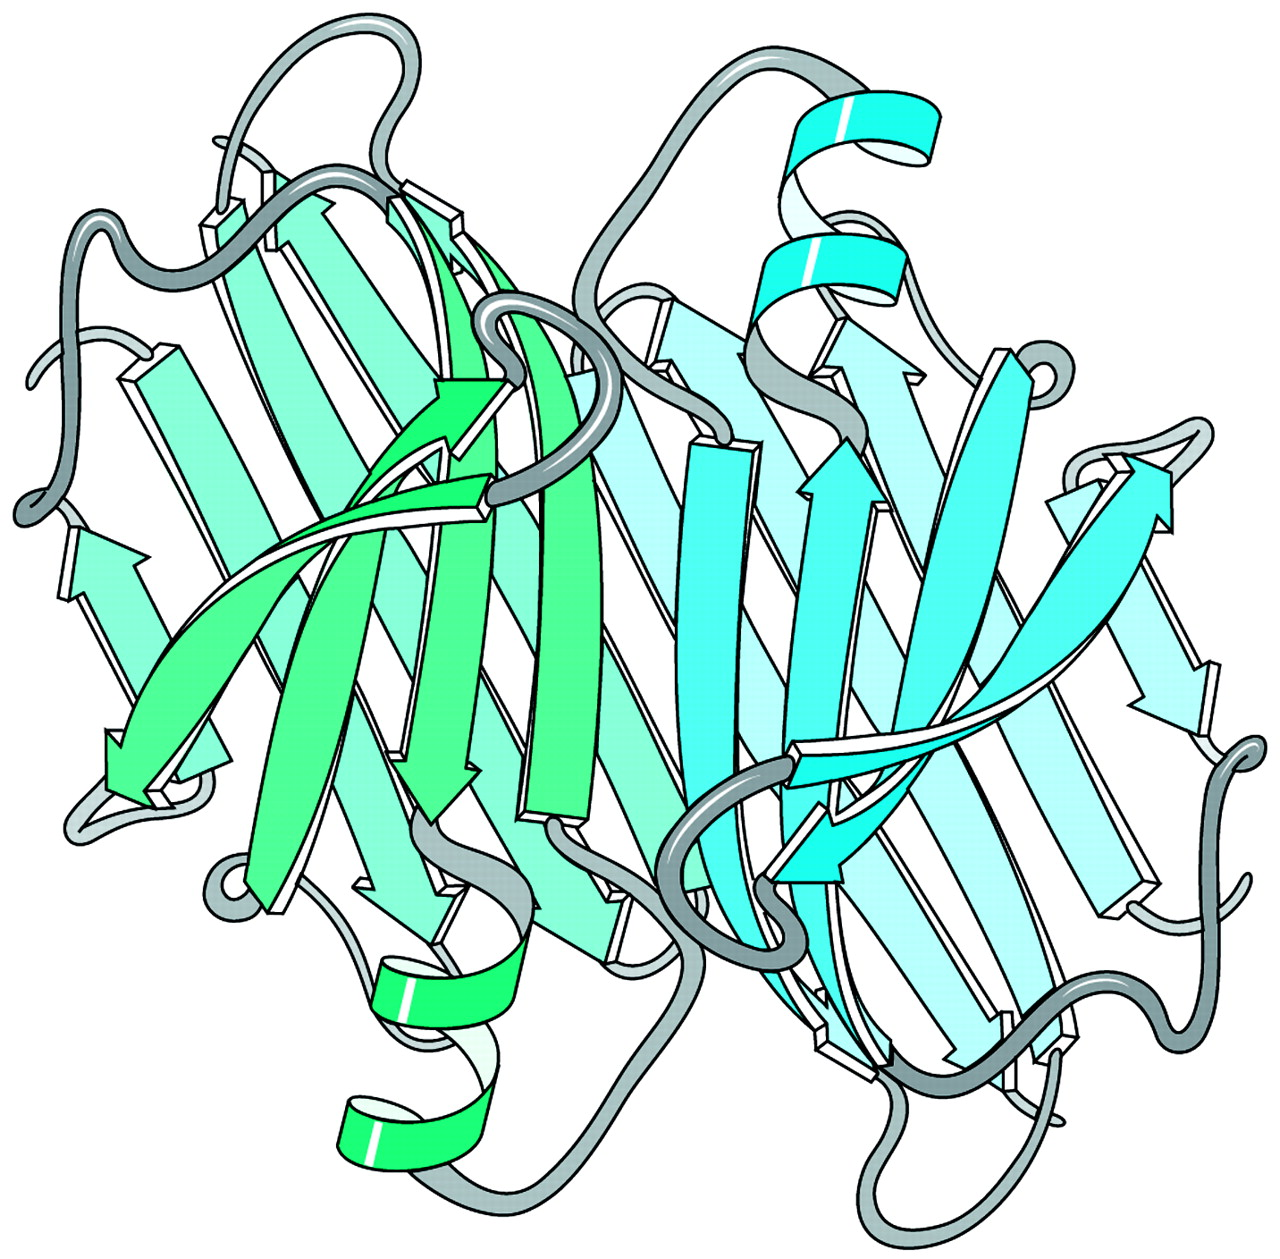
\includegraphics[scale=0.4]{Chapter1/overallfold.png}
\caption{Ribbon-coil    schematic    illustraring    the   fold    and
  intermolecular  units of  a dimer  of prealbumin  (PDB\_ID:2PAB), or
  transthyretin,    taken     from    Richardson    \textit{et    al.}
  \cite{richardson2002}}
\label{fig:ribboncoil}
\end{figure}

\begin{figure}[t]
\centering
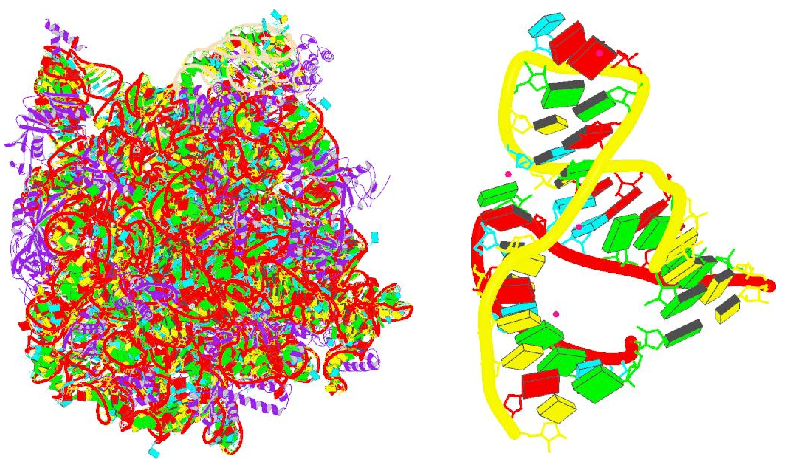
\includegraphics[scale=0.5]{Chapter1/ribosome_ribozyme.png}
\caption{Images   of  the  \textit{Haloharcula   marismortui's}  large
  ribosomal subunit NDB\_ID:RR0033 (left) and the hammerhead ribozyme
  (right) NDB\_ID:UR0029.
  The  figures were taken directly  from the NDB
  web  pages,   and  show  a  3DNA-generated  \cite{lu2008b}  ribbon
  representation of the phosphate backbone, and a block representation
  of the nucleotide bases. From  the figures is clear that, whereas
  the   ribozyme   fold   can   be  clearly   understood   with   this
  representation, the ribosome fold cannot.}
\label{fig:ribosome}
\end{figure}

One  can  envision that  a  thorough  investigation  of the  space  of
translational and rotational degrees of freedom of the helical regions
of RNA could give clues as to  how one might see an overall fold in RNA
structures.  To the  best  of  our knowledge,  there  is no  comparable
quantitative description of the folding of proteins.

In  the  case  of  proteins,  the SCOP  (Structural  Classification  of
Proteins)  database  \cite{andreeva2004}  classifies  proteins,  among
various  qualitative  descriptors,   according  to  folds,  which  are
recurrent  arrangements of  secondary structure,  that is,  a  list of
consecutive secondary structures  with unique topological connections.
The    SCOR    (Structural    Classification    of    RNA)    database
\cite{klosterman2002,  klosterman2004}  aims   to  provide  a  similar
classification  to that obtained  for proteins,  but using  RNA motifs
instead.  This  classification focuses on  the local folding  of small
pieces  of  RNA  and  does not  describe the  overall  fold.  The  local
classification of RNA  motifs in SCOR is also  qualitative rather than
quantitative.

\subsection{RNA motifs}
The term ``\textit{RNA motif}'' is  used in the literature to describe
three   different   levels    of   RNA   organization,   namely,   RNA
\textbf{sequence} motifs, RNA  \textbf{secondary structure} motifs, or
RNA \textbf{3D structure} motifs.   Because these distinctions are not
always clearly  made, the beginner may become  confused and frustrated
in bibliographical searches.

The lack of a unique definition of RNA motifs is yet another source of
confusion.  Three  popular and  somewhat  recent  definitions of  RNA
motifs include:
\begin{itemize}
\item{``\textit{a discrete sequence or combination of
    base  juxtapositions   found  in  naturally   occurring  RNA's  in
    unexpectedly high abundance.}''\cite{moore1999}}
\item{``\textit{conserved structural subunits that make
    up the secondary structures of RNAs.}''\cite{holbrook2005}}
\item{``\textit{ordered   stacked    arrays   of
    non-Watson-Crick  base  pairs  that  form distinct  folds  on  the
    phosphodiester backbones of RNA strands.}''\cite{leontis2003}}
\end{itemize}

The  kind of RNA  motifs addressed in this
thesis are of the third type, that is, RNA \textbf{3D structure}
motifs  which we henceforth term RNA  motifs.
From our point of view, RNA motifs are to be understood as  unique
sets of geometrical  arrangements (in the rigid block sense) in
three-dimensional space.

Even  though there  is no  unique definition,  we can  think  of three
practical  tasks regarding  RNA  motifs.   That is,  given  an RNA  3D
structure, automatically identify, describe,  and find new motifs.  For
automatic  identification of  RNA motifs,  Pyle and  collaborators have
developed  the AMIGOS software, which finds  RNA motifs
based on  specific values of the backbone virtual  torsion angles $\eta$
and  $\theta$  \cite{olson1980, malathi1985,  duarte2003} in  a  way  which
resembles   a   Ramachandran  plot   analysis.    Lemieux  and   Major
\cite{lemieux2006}  employ  the  MC-Fold software,  which  implicitly
finds RNA motifs based on  an algorithm that determines so-called nucleic
cyclic  motifs, which  are  just the  minimal  cycle basis  of an  RNA
secondary  structure  interpreted as  a  mathematical graph.   Leontis
\cite{nasalean2009}  and collaborators have created FR3D  (read  as FRED),
a Matlab  Windows executable program  which finds  RNA motifs
based on the isostericity matrices of base-pairs.

Schlick and collaborators have used FR3D
to  localize  RNA helical  junctions  of  order  four (i.e.   four-way
junctions) or  higher, and performed a  visual analysis to  see if the
helices  in  such junctions  form  coaxial  stacks  or not,  and  have
classified   them   accordingly   \cite{laing2009,  laing2009a}.    As
mentioned previously in the context of RNA folds, Holbrook, and Sykes,
describe   helical  regions  and   display  them   in  two-dimensional
representations. Sponer's group has studied  RNA
motifs present  in the ribosome using Molecular  Dynamics (MD) methods
implemented  in   the  AMBER   package,   including 25ns
simulations  of   the  sarcin-ricin  domain  (SRD)
\cite{spackova2006},  and 80ns simulations  of the  hydration of
loop E in the 5S subunit \cite{reblova2003}.

The software programs, which perform the task of identifying RNA motifs
in RNA structures - namely AMIGOS, MC-Fold, and FR3D - also have the
capability to find new RNA motifs.

\section{Overview}
Keeping always in  mind the greater scope of  the RNA folding problem,
this thesis  addresses various issues of  RNA structural understanding
using RNA crystallographic data from the Protein Data Bank (PDB). Such
data  have been  analyzed statistically  in terms  of a rigourous
rigid-body formalism.  In Chapter 2 the consensus clustering technique
is   used  to   classify   RNA  base-step   parameters  of   non-A-RNA
conformations, and  the resulting groups are  localized and examined
in the context  of rRNA.  Chapter 3 reconsiders  previous work carried
out by  Dr. Yurong Xin  in Dr. Olson's group lab, on classification  of RNA
base-pairs, by  resorting the structures in her base pair structures
(BPS) database with clustering  analysis techniques.
In  Chapter 4 we  explore, using statistical  analyses, the
data available for RNA  helical regions, and  use the  information to
determine the persistence length and elastic behaviour of
double-stranded RNA's with various repeating sequences and compare the
crystallographic based behaviour with other experimental  results.  In
Chapter  5 we  provide  a  new  python
software,  pyRNAmotifs which interfaces  with 3DNA  to perform a rigourous
search of existing and perhaps  new RNA motifs, and finally in Chapter
6  we propose  the measurement  and classification  of  RNA structures
using a  new graph theoretical index  named folding index,  based on a
helical region "view"  of RNA's, which is clearly  concordant with the
emerging  necessity   of  new  metrics  beyond   RMSD  for  structural
understanding.

\bibliography{biblio}
